\documentclass[12pt]{article}       % 設定文件類型為 article,字體大小為 12pt
\usepackage[T1]{fontenc}            % 設定 T1 字型編碼,確保特殊字元的正確顯示
\usepackage{lmodern}                % 強制使用 Latin Modern 字型,提高可讀性和相容性
\usepackage{fontspec}               % 允許使用 OpenType 和 TrueType 字型
\usepackage{graphicx}               % 支援插入圖片
\usepackage{amsmath}                % 提供數學環境和公式支持
\usepackage{csquotes}               % 提供引用格式支援
\usepackage{comment}                % 提供多行註解
\usepackage{ragged2e}

%biber NSTC_project

%=================================================={{{參考文獻設定}}}==================================================

\usepackage[style=ieee, maxnames=99]{biblatex}          % 設定參考文獻格式為 IEEE,最多顯示 99 個作者
\addbibresource{NSTC_project.bib}                       % 添加參考文獻檔案 references.bib
\renewcommand{\bibfont}{\fontspec{Times New Roman}}     % 設定參考文獻字體為 Times New Roman
\renewcommand{\UrlFont}{\fontspec{Times New Roman}}     % 設定 URL 連結字體為 Times New Roman
\DeclareFieldFormat{url}{\url{#1}}                      % 格式化 URL
\bibliography{your_bib_file}                            % 引用你的 .bib 文件

%=================================================={{{目錄設定}}}==================================================

\usepackage{tocloft}                                            % 自訂目錄格式

% 設定目錄的點線填充樣式
\renewcommand{\cftsecleader}{\cftdotfill{\cftdotsep}}           % 節(section)
\renewcommand{\cftsubsecleader}{\cftdotfill{\cftdotsep}}        % 小節(subsection)
\renewcommand{\cftsubsubsecleader}{\cftdotfill{\cftdotsep}}     % 子小節(subsubsection)

% 設定目錄標題格式
\renewcommand{\contentsname}{\centering \LARGE \textbf{目錄}}    % 目錄標題置中,字體大小為 LARGE,加粗

%=================================================={{{字體設定}}}==================================================

% 設定英文字體
\newfontface\englishfont{Times New Roman}               % 自訂英文字體命令 \englishfont,使用 Times New Roman

\setmainfont[
    ItalicFont={Times New Roman Italic},                % 設定斜體
    BoldFont={Times New Roman Bold},                    % 設定粗體
    BoldItalicFont={Times New Roman Bold Italic}        % 設定粗斜體
]{Times New Roman}                                      % 設定主要英文字體為 Times New Roman

% 設定中文字體

\usepackage{xeCJK}                                      % 使用 xeCJK 宏包以支援中文
\renewcommand{\figurename}{圖}                           % 設定圖表名稱
\setCJKmainfont[BoldFont={標楷體-繁}, ItalicFont={標楷體-繁}] {標楷體-繁}

%=================================================={{{版面設定}}}==================================================

% 設定頁面邊界,適用 A4 紙張
\usepackage[top=2cm, bottom=2cm, left=2cm, right=2cm, a4paper]{geometry}

% 設定行距與段落格式
\usepackage{setspace}
\onehalfspacing % 設定 1.5 倍行距
\setlength{\parskip}{6pt} % 設定段落間距 6pt
\setlength{\parindent}{2em} % 設定段落首行縮排 2 個字元

%=============================================================================================================================
%=============================================================================================================================
%=============================================================================================================================

\begin{document}

\pagenumbering{roman}  
\setcounter{page}{1}  % 從 I 開始

%=================================================={{{中文摘要}}}==================================================

\section*{\centering 摘要}  % 只讓標題置中
\addcontentsline{toc}{section}{摘要}  % 手動加入摘要到目錄

%==============================摘要內容==============================

\hspace{2em}
本研究計畫旨在開發一套智慧交通巡檢系統,利用四軸飛行載具(Unmanned Aerial Vehicle, UAV)進行違規停車車輛的偵測。
不同於以往先判斷紅線位置再確認車輛是否違規的方法,本研究透過四軸飛行器的GPS定位資訊來判斷車輛是否違規,避免車輛停在紅線上或完全遮掩紅線的情況。
由於系統僅檢視違規區域,此方法還能加快巡邏速度,提升巡邏效率。

本系計畫統採用YOLOv7物件偵測模型進行即時車輛辨識,結合飛行器的姿態與相機拍攝角度,
利用透視變換(Perspective Transformation)定位,將偵測結果轉換為地面上的絕對位置,這樣能夠快速確定違規停車車輛的位置。
透過事先建立的資料庫,無人機將比對飛越指定區域所拍攝的影像,並即時偵測違規車輛,記錄其位置。
該系統的優勢在於高效的監控能力,能夠大幅減少設備投資成本,並提升違規車輛檢測的靈活性和即時性。

\vspace{1.5em}
\noindent 關鍵字:即時物件偵測、四旋翼無人機、空間對位
%==============================摘要內容==============================
\newpage  % 插入換頁命令,將目錄和後續內容分開

%=================================================={{{英文摘要}}}==================================================
\section*{\centering Abstract}  % 只讓標題置中
\addcontentsline{toc}{section}{Abstract}  % 手動加入摘要到目錄
%==============================摘要內容==============================
\hspace{2em}This research aims to develop an intelligent traffic inspection system utilizing unmanned aerial vehicles (UAVs) to detect illegally parked vehicles.
Unlike conventional methods that first identify the location of red lines and then verify whether vehicles are violating parking regulations, this system determines whether a vehicle is in violation by using the UAV's GPS positioning information, preventing vehicles from parking on or completely covering red lines.
Since the system only inspects the violation areas, this approach helps speed up patrol operations and enhance overall patrol efficiency.

This research adopts the YOLOv7 object detection model for real-time vehicle identification, combined with the UAV's attitude and camera angle.
By using perspective transformation, the system locates and converts the detection results into absolute ground positions, allowing for quick identification of illegally parked vehicles.
Through a pre-established database, the UAV compares the images captured while flying over designated areas and immediately detects violation vehicles, recording their locations. The advantage of this system lies in its efficient monitoring capability, significantly reducing equipment investment costs and improving the flexibility and immediacy of illegal parking detection.

\vspace{1.5em}
\noindent Keyword: Real-time Object Detection, Quadcopter, Georeferencing
%==============================摘要內容==============================
\newpage  % 插入換頁命令,將目錄和後續內容分開

%=================================================={{{目錄}}}==================================================

\begin{center}
\tableofcontents  % 插入目錄,並置中
\thispagestyle{empty}  % 讓目錄頁沒有頁碼
\end{center}
\newpage  % 插入換頁命令,將目錄和後續內容分開

%=================================================={{{內容開始}}}==================================================

\pagenumbering{arabic}  % 開始使用阿拉伯數字頁碼
\setcounter{page}{1}  % 設定頁碼從 1 開始

%\englishfont{this is an example of mixed English and Chinese.}

\section{\centering 緒論}

\subsection{研究背景} 
%==============================內文==============================
\hspace{2em}
無人機(Unmanned Aerial Vehicle, UAV)技術近年來快速發展,整合各種附加設備並隨著飛行控制與自動化技術的成熟,在軍事、執法及科技應用領域取得顯著成效。
四軸旋翼無人機因其安全性高、成本低的優勢,已廣泛應用於各種場景,其中攝影與錄影功能尤為重要。
無人機擁有比傳統攝影設備更廣的視角,且受環境限制較小,使其在大範圍場景捕捉方面表現優異,優於傳統監控方式。

在交通監控領域,無人機的靈活性和效率遠勝於傳統固定式監控設備,如固定式照相桿雖能執行監控任務,但監測範圍有限且設備成本較高。
隨著無人機技術的進步,其在交通巡檢方面展現出極大的應用潛力,特別是在違規停車偵測方面,無人機能夠提供更靈活且高效的解決方案。
目前,中國部分城市已開始運用無人機進行科技執法\cite{chinatimes2019},台北市與台中市警察局亦已成立無人機機隊\cite{cna_2022}\cite{tai_2021},用於交通監測與執法,並協助執法人員即時掌握交通狀況,提升執法效率。

\begin{figure}[htbp]
    \centering
    \renewcommand{\figurename}{圖} %顯示圖1,不是figureat1
    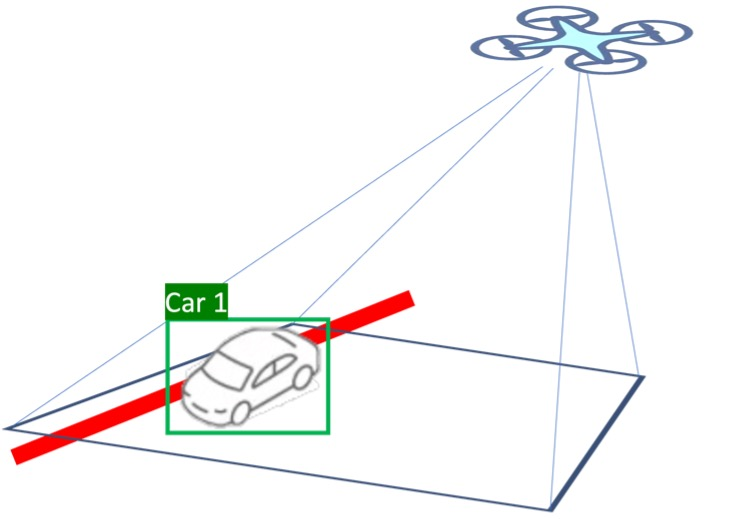
\includegraphics[width=0.7\textwidth]{research_problem1.jpg}     %圖片檔案名稱
    \caption{無人機偵測違停車輛示意圖}    %圖片檔案名稱
    \label{fig:research_problem1}    %為圖片添加標籤
    %圖\ref{fig:無人機偵測違停車輛示意圖}
\end{figure}
%==============================內文==============================

\subsection{研究動機} 
%==============================內文==============================
\hspace{2em}目前的研究和應用大多針對車輛橫跨紅線進行判斷,但對於完全蓋住紅線或停在紅線與白線交界處的情況,現有方法無法準確判斷車輛是否違停。
因此,本研究計畫的動機在於利用無人機的GPS位置資訊來判斷車輛的違規情形,避免車輛完全遮掩紅線或停在紅線邊界處的情況。
如圖\ref{fig:research_problem2}所示。
並通過建立資料庫並使用無人機拍攝影像,比對車輛所處位置與違規區域,能夠快速偵測違規車輛並進行即時回報,進一步提升交通執法的效率與靈活性。

\begin{figure}[htbp]
    \centering
    \renewcommand{\figurename}{圖} %顯示圖1,不是figureat1
    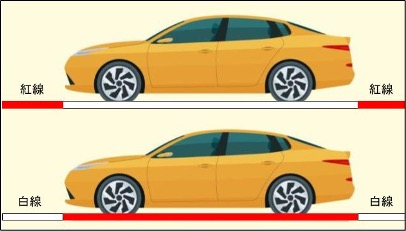
\includegraphics[width=0.7\textwidth]{research_problem2.jpg}     %圖片檔案名稱
    \caption{本計畫研究問題之示意圖}    %圖片檔案名稱
    \label{fig:research_problem2}    %為圖片添加標籤
    %圖\ref{fig:example1}
\end{figure}
%==============================內文==============================

\subsection{研究問題} 
%==============================內文==============================
\hspace{2em}利用無人機拍攝出的影像辨識出沿路車輛,利用無人機本身 GPS 位置,換算出影像中車輛之位置,比對車輛所在位置是否可以停車,
以判斷車輛否違規,若有違規情形,回傳車輛位置並將其建立成資料庫,以便於人員複查或是違規檢舉。研究問題可以分為三大項,違規車輛偵測、影像處理、空間對位。


%==============================內文==============================

\subsubsection{違規車輛偵測}
%==============================內文==============================
\hspace{2em}為了精確偵測違規停放的車輛,本系統採用先進的影像辨識技術,利用 YOLOv7 進行即時車輛偵測,確保能快速且準確地識別影像中的車輛。
透過無人機高空巡檢,可大範圍覆蓋監控區域。此外,系統將結合 GPS 位置資訊,以判斷車輛是否位於可能的違規區域,
如紅線停車區、消防通道或人行道上,進一步提高偵測的可靠性與準確性。
%==============================內文==============================

\subsubsection{影像處理}
%==============================內文==============================
\hspace{2em}本計畫將利用鏡頭往斜下的角度拍攝而非垂直向下。以斜下角度拍攝的特點是相較於垂直向下拍攝可以擁有較大的視野範圍。
而採用無人機的 GPS位置資訊判斷,無人機拍攝圖片中每個像素與實際地面之關係格外重要,除了無人機上相機的傾角,
還需整合無人機在飛行時的對地高度、翻滾角 (Roll)、俯仰角(Pitch)、偏航角(Yaw)等慣性測量單元(Inertial measurement unit, IMU),
並依據該照片拍攝時之IMU資訊做正射投影,運算每個像素與無人機之間的相對位置,並依照無人機的GPS位置準確定位違規車輛之位置。
%==============================內文==============================

\subsubsection{空間對位}
%==============================內文==============================
\hspace{2em}為確保偵測結果的精準性,系統將進行空間對位處理,以克服飛行器姿態變化、鏡頭視角與透視變形等因素所造成的誤差。
透過飛行器的 IMU(慣性測量單元)數據與 GPS 定位資訊,獲取無人機的姿態與拍攝角度,並利用透視變換技術將影像坐標轉換為地面絕對位置。
最後,系統將偵測出的車輛位置與電子地圖上的違規區域進行重合度分析,精確確認車輛是否確實違規停放,並輸出違規證據以供後續處理。
%==============================內文==============================

\section{\centering 文獻探討與回顧}
%==============================內文==============================
\hspace{2em}


%==============================內文==============================


\section{\centering 研究方法及流程}
%==============================內文==============================
\hspace{2em}


%==============================摘要內容==============================


\section{\centering 研究結果}
%==============================摘要內容==============================



%==============================摘要內容==============================


\section{\centering 結論} 
%==============================摘要內容==============================



%==============================摘要內容==============================

\section{\centering 參考文獻}
\vspace{-3.5em}  % 減少與上方內容的間距
\renewcommand{\refname}{}  % 去除 "References" 標題
\printbibliography  % 列出參考文獻

\end{document}

%=============================================================================================================================
%=============================================================================================================================
%=============================================================================================================================


\begin{comment}
    %==============================圖片==============================
    \begin{figure}[h]
        \centering
        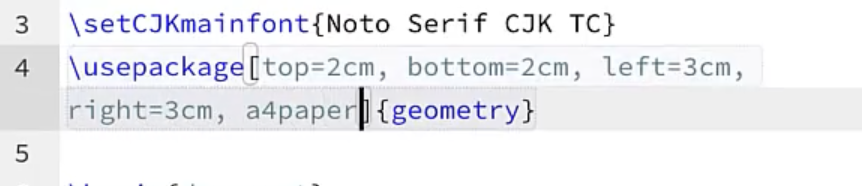
\includegraphics[width=0.7\textwidth]{截圖 2025-01-24 03.21.17.png}     %圖片檔案名稱
        \caption{這是圖片的標題}    %圖片檔案名稱
        \label{fig:example2}    %為圖片添加標籤
        %如\ref{fig:example1}所示
    \end{figure}
    
    %==============================數學公式==============================
    \begin{align}
        a &= b + c \label{eq:1}
        \\
        d &= e - f \label{eq:2}
        %式label{eq:2}
    \end{align}
    
    %==============================表格==============================
    \begin{table}[ht]
        \centering
        \begin{tabular}{|c|c|c|}
        \hline
        項目  & 數量 & 價格 \\
        \hline
        蘋果  & 10  & 30   \\
        香蕉  & 5   & 15   \\
        橙子  & 8   & 20   \\
        \hline
        \end{tabular}
        \caption{水果表格}
        \label{tab:fruits}
    \end{table}
    
    \end{comment}
        